\section{Das Tschebyscheff - Verfahren}

\begin{defn}
Mit $E(f_1,f_2,\rho)$ bezeichnen wir die Ellipse mit den Brennpunkten $f_1$, $f_2$ und den Halbachsen $
\frac{1}{4}\left|f_1-f_2\right|\left(\rho + \frac{1}{\rho}\right)$
und  $\frac{1}{4}\left|f_1-f_2\right|\left(\rho - \frac{1}{\rho}\right)$,
$\rho \ge 1$.
\end{defn}

Wir betrachten nun folgende Situation:

\medskip

\emph{Gegeben: } $Ax = b$, $A$ regul"ar.

\emph{Bekannt sei:} $\spek(A) \subseteq E(f_1,f_2,\rho)$ mit $0 \not \in E(f_1,f_2,\rho)$.

\begin{figure}[h!]
\begin{center}
\begin{picture}(250,100)
\unitlength1pt
\rput{34}{\psellipse(160pt,-25pt)(50pt,25pt)\qdisk(185pt,-25pt){2pt}\qdisk(135pt,-25pt){2pt}}
\put(0,50){\vector(1,0){200}}
\put(60,0){\vector(0,1){100}}
\end{picture}
\end{center}
\caption{$\spek(A)$ liegt in einer Ellipse, welche 0 nicht enth"alt}
\end{figure}

Mit Hilfe der Tschebyscheff-Polynome werden wir (asymptotisch optimale) N"aherungsl"osungen
f"ur die MinMax-Aufgabe
\begin{equation} \label{minmaxell2_eq}
\underset{p_m \in \overline{\Pi}_m \quad}{\min}\underset{\lambda \in E(f_1,f_2,\rho)}{\max}\left| p_m(\lambda)\right|
\end{equation}
finden. Daf"ur ben"otigen wir zun"achst die affine Transformation, welche
unsere Standard-Ellipse $E_{\rho} = E(-1,1,\rho)$ auf $E(f_1,f_2,\rho)$  abbildet.

Wir betrachten hierzu die affinen Grundabbildungen
\begin{align*}
D_{ \phi}&: z \mapsto e^{i \phi}z, \phi \in \rr \enspace (\text{Drehung})\\
T_a&:z \mapsto z + a, a \in \co \enspace (\text{Translation})\\
S_c&: z \mapsto cz, c >0 \enspace (\text{Skalierung})
\end{align*}

\begin{lem}\label{ellipsentransf_lem} 
Die Abbildung
\begin{eqnarray*}
\varphi &=& T_{\frac{1}{2}(f_1+f_2)} \circ D_{\arg(f_2-f_1)} \circ S_{\frac{1}{2}\left| f_1
- f_2 \right|} \\
\varphi&:& z \mapsto e^{i \arg(f_2-f_1)}\frac{1}{2} \left| f_2-f_1 \right| z +
    \frac{f_1+f_2}{2} = \underbrace{\frac{f_2-f_1}{2}}_{\alpha} z + \underbrace{\frac{f_1+f_2}{2}}_{\beta}
\end{eqnarray*}
bildet die Ellipse $E(-1,1,\rho)$ ab auf $E(f_1,f_2,\rho)$. 
\end{lem}

Damit k�nnen wir nun Tschebyscheff Polynome  bez"uglich allgemeiner
Ellipsen $E(f_1,f_2,\rho)$ definieren.

\begin{defn}
Sei $E=E(f_1,f_2,\rho)$ eine Ellipse mit $0 \not \in E$. Dann ist
\[
T_m^E(z) = T_m \left( \frac{1}{\alpha}(z- \beta) \right)
\]
mit $\alpha = \frac{1}{2}\left( f_2 - f_1 \right) $ und 
$ \beta = \frac{1}{2} \left( f_1 + f_2 \right)$ das
\emph{Tschebyscheff-Polynom} vom Grad $m$ bzgl. $E$. 
\end{defn}

Nach Satz \nref{cmschranke_sa} ist damit klar, dass
\[
p_m(z)=\frac{T_m^E(z)}{T_m^E(0)}
\]
eine approximative, asymptotisch optimale, L�sung f�r die MinMax-Aufgabe
\eqnref{minmaxell2_eq} ist.

\begin{defn}
Das zu $p_m$ geh�rige KUV hei�t \emph{Tschebyscheff-Verfahren}.
\end{defn}

Wir werden nun dieses Verfahren konkret herleiten. Hierf�r betrachten wir den Fall 
einer allgemeinen 3-Term-Rekursion
\[
p_{m+1}(t) = \alpha_{m+1}(t+\beta_{m+1})p_{m}(t) + \gamma_{m+1}p_{m-1}(t) \text{, } m \ge 1.
\]
Wegen $p_m(0) = 1,\; \forall\ m,$ folgt $\gamma_m = 1- \alpha_m \beta_m$
und insbesondere
\[
 p_0(t) = 1, \enspace p_1(t) = \alpha_1 \left (t+ \frac{1}{\alpha_1} \right ).
\]
Es gilt also f�r die Residuen $r^m = b - Ax^m = p_m(A)r^0$
\begin{align*}
r^{m+1} &= \alpha_{m+1}(A + \beta_{m+1} I) r^m+(1- \alpha_{m+1} \beta_{m+1})r^{m-1} \text{, } m \ge 1, \\
r^0 &= r^0, \\
r^1 &= \alpha_1\left(A + \frac{1}{\alpha_1} I\right) r^0 = \alpha_1 A r^0 + r^0.
\end{align*}
Damit erhalten wir f"ur die Iterierten unter Einsetzen von $r^m = b-Ax^m$ die Rekursion
\begin{align*}
x^0 &= x^0, \\
x^1 &= x^0 - \alpha_1 r^0 ,\\
x^{m+1} &= \alpha_{m+1} \beta_{m+1} x^m + (1- \alpha_{m+1} \beta_{m+1})x^{m-1} - \alpha_{m+1} r^m.
\end{align*}

Damit erhalten wir als allgemeine Struktur f�r ein KUV mit 3-Term-Re\-kur\-sion f�r die Residuen den folgenden Algorithmus:
\clearpage
\begin{alg} \label{3Term_alg}
~  				% um "3.4 Algorithmus" aus dem Kasten rauszubekommen
\vspace*{-2\baselineskip}	% um den Leeraum zu entfernen
\begin{algorithm}
\begin{algorithmic}
\STATE w�hle $x^0$, setze $r^0 = b -Ax^0$
\STATE $x^1 = x^0 - \alpha_1 r^0$
\STATE $r^1 = \alpha_1 A r^0 + r^0$ 
\FOR{$m=1,2,...$}
\STATE $x^{m+1}= \alpha_{m+1} \beta_{m+1} x^m + (1 - \alpha_{m+1} \beta_{m+1}) x^{m-1} - 
      \alpha_{m+1} r^m$
\STATE $r^{m+1}=b-Ax^{m+1}$ 
\ENDFOR
\end{algorithmic}
\end{algorithm}
\end{alg}

(Alternativ k�nnte man $r^{m+1}$ auch aus der 3-Term-Rekursion bestimmen)



%\makeatletter

%\makeatother

%%

Jetzt geht es um die konkrete Bestimmung der Koeffizienten
$\alpha_m$, $\beta_m$ beim Tschebyscheff-Verfahren.

Mit $E=E(f_1,f_2,\rho)$, $a=\frac{1}{2}(f_2-f_1)$ und
$b=\frac{1}{2}(f_2+f_1)$ gilt
\[
  T_m^E(z)=T_m\left(\frac{1}{a}(z-b)\right).
\]
Es gilt $T_0(z)=1$, $T_1(z)=z$ und $T_{m+1}(z)=2zT_m(z)-T_{m-1}(z)$. Also folgt
\begin{align*}
T_0^E(z)&=1,\\
T_1^E(z)&=\frac{1}{a}(z-b)\\
\text{und}\qquad
T_{m+1}^E(z)&=T_{m+1}\left(\frac{1}{a}(z-b)\right)
=\frac{2}{a}(z-b)T_m^E(z)-T_{m-1}^E(z).
\end{align*}
Die Residuenpolynome $p_m(z)$ f"ur das Tschebyscheff-Verfahren sind
\[
 p_m(z)=\frac{T_m^E(z)}{T_m^E(0)}.
\]
Wir ben"otigen also $c_m:=T_m^E(0)$ und finden
\begin{equation}
  \label{TschVerf-c-m+1}
  \left\{ \quad
  \begin{aligned}
    c_0 &= 1, \\
    c_1 &= -\frac{b}{a} \\
    \text{und}\qquad
    c_{m+1} &= -\frac{2}{a}bc_m-c_{m-1}, \; m\geq 1.
  \end{aligned}
  \right.
\end{equation}
Damit erhalten wir
\begin{align*}
  p_0(z) &= 1, \\
  p_1(z) &= -\frac{1}{b}(z-b) \\
  \text{und}\qquad
  p_{m+1}(z) &= \frac{1}{c_{m+1}}\left(
    \frac{2}{a}(z-b)c_mp_m(z)-c_{m-1}p_{m-1}(z)
  \right), \; m\geq 1.
\end{align*}

\begin{bem}
  Es gibt verschiedene andere Formulierungen, mit denen die Koeffizienten
  aufdatiert werden k"onnen. Die Werte $c_m$ werden schnell sehr gro"s;
  deshalb ist es aus numerischen Gr�nden besser, die Berechnung von
  $c_{m+1}$ zu vermeiden, und daf�r die Quotienten $\delta_{m+1}=
  \frac{c_{m+1}}{c_m}$ aufzudatieren. Wir erhalten
  \[
  \frac{c_{m+1}}{c_m}=-\frac{2}{a}b-\frac{c_{m-1}}{c_m},
  \]
  und damit
  \begin{align*}
    \delta_1&=c_1\\
    \text{und}\qquad
    \delta_{m+1}&=-\frac{2}{a}b-\delta_m^{-1}, \; m \geq 0.
  \end{align*}
\end{bem}
Wegen $\frac{c_{m-1}}{c_{m+1}} = 1 - \frac{2b}{a}\frac{c_m}{c_{m+1}}$ (dies gilt,
da $p_m(0)=1$ f"ur alle $m$) ergibt sich
\begin{align*}
  p_0(z) &= 1, \\
  p_1(z) &= -\frac{1}{b}(z-b) \\
  \text{und}\qquad
  p_{m+1}(z) &=
  \frac{2}{a\delta_{m+1}}(z-b) p_m(z)
  - \left( 1 - \frac{2b}{a\delta_{m+1}} \right) p_{m-1}(z).
\end{align*}

Die Koeffizienten der 3-Term-Rekursion sind also
\[
  \alpha_{m} = \frac{2}{a\delta_m}, \; \beta_m = -b; m \geq 2.
\]

Damit erhalten wir den folgenden Algorithmus f"ur das Tschebyscheff-Ver\-fahren
zur L�sung von $Ax = c$ ($b$ ist schon vergeben \ldots):
\clearpage

\begin{alg} \label{Tschebyscheff_alg}
~                               		% um "x.x Algorithmus" aus dem Kasten rauszubekommen
\vspace*{-2\baselineskip}       % um den Leeraum zu entfernen
\begin{algorithm}[Tschebyscheff-Verfahren]
%  \caption{Tschebyscheff-Verfahren}
  \begin{algorithmic}
    \REQUIRE $\spek(A)\subseteq E(f_1,f_2,\rho)\not\ni 0$
    \STATE setze $a=\frac{1}{2}(f_2-f_1)$, $b:=\frac{1}{2}(f_2+f_1)$
    \STATE setze $\delta_1=-b/a$
    \STATE w�hle $x^0$
    \STATE setze $r^0=c-Ax^0$
    \STATE $\alpha_1=-2/b$
    \STATE $x^1=x^0-\alpha_1r^0$
    \STATE $r^1=\alpha_1Ar^0+r^0$
    \FOR{$m=1,2,\dots$}
    \STATE $\delta_{m+1}=-\frac{2}{a}b-1/\delta_m$
    \STATE $\alpha_{m+1}=2/(a\cdot\delta_{m+1})$
    \STATE $x^{m+1}=(-\alpha_{m+1}b)x^m+(1+\alpha_{m+1}b)x^{m-1}
    -\alpha_{m+1}r^m$
    \STATE $r^{m+1}=c-Ax^{m+1}$
    \ENDFOR
  \end{algorithmic}
\end{algorithm}
\end{alg}

\begin{bem}
  Wegen $p_m(0)=1$ muss auch gelten
  \begin{equation*}
    1=\frac{c_m}{c_{m+1}}\cdot\frac{2}{a}(-b)-\frac{c_{m-1}}{c_{m+1}},
  \end{equation*}
  was man mit \eqref{TschVerf-c-m+1} best"atigt.
\end{bem}

\begin{aufg}
  Implementiere das Tschebyscheff-Verfahren f�r das Modellproblem~I
  f�r verschiedene Gittergr��en $N$.

  Verwende dabei $\spek(A)\subseteq[\xi,\Xi]$ mit
  \begin{align*}
    \xi &= 4-4\cos(\pi h),  \qquad  h=\frac{1}{N+1},\\
    \text{und}\qquad
    \Xi &= 4+4\cos(\pi h).
  \end{align*}
  Die zugeh�rige Ellipse ist also
  \begin{equation*}
    E(\xi,\Xi,1)
  \end{equation*}
  \begin{itemize}
  \item Plotte $\norm{r^m}$ gegen $m$ f�r verschiedene Werte von $N$.
  \item Teste auch $2\Xi$ statt $\Xi$ (langsamere Konvergenz).
  \item Teste auch $\Xi-\xi$ statt $\Xi$ (keine Konvergenz).
  \item Teste auch $\xi+10 \cdot h^2$ statt $\xi$ .
  \item Teste auch $\frac{\xi+ \Xi}{2}$ statt $\xi$ (langsamere Konvergenz).
\end{itemize}
\end{aufg}

\begin{figure}
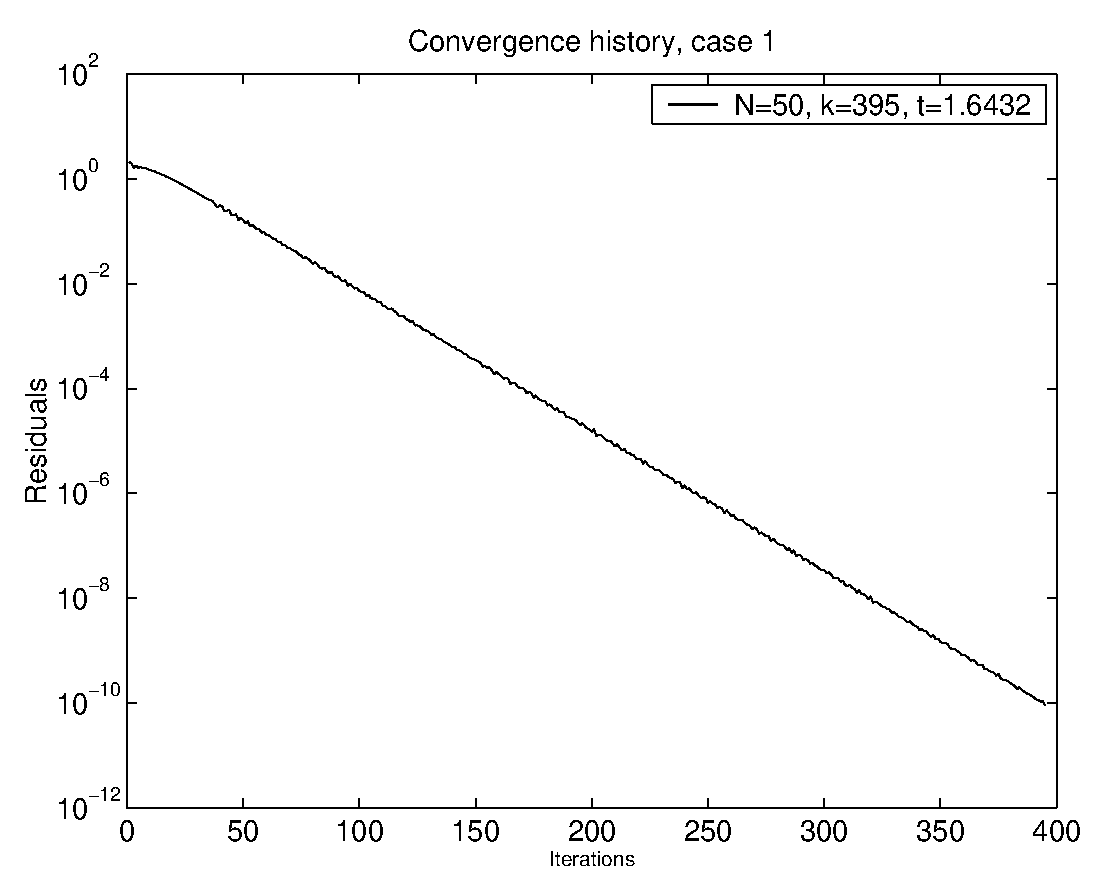
\includegraphics[scale=0.35]{eps/tscheb1.eps}\hfill\includegraphics[scale=0.35]{eps/tscheb2.eps} \\
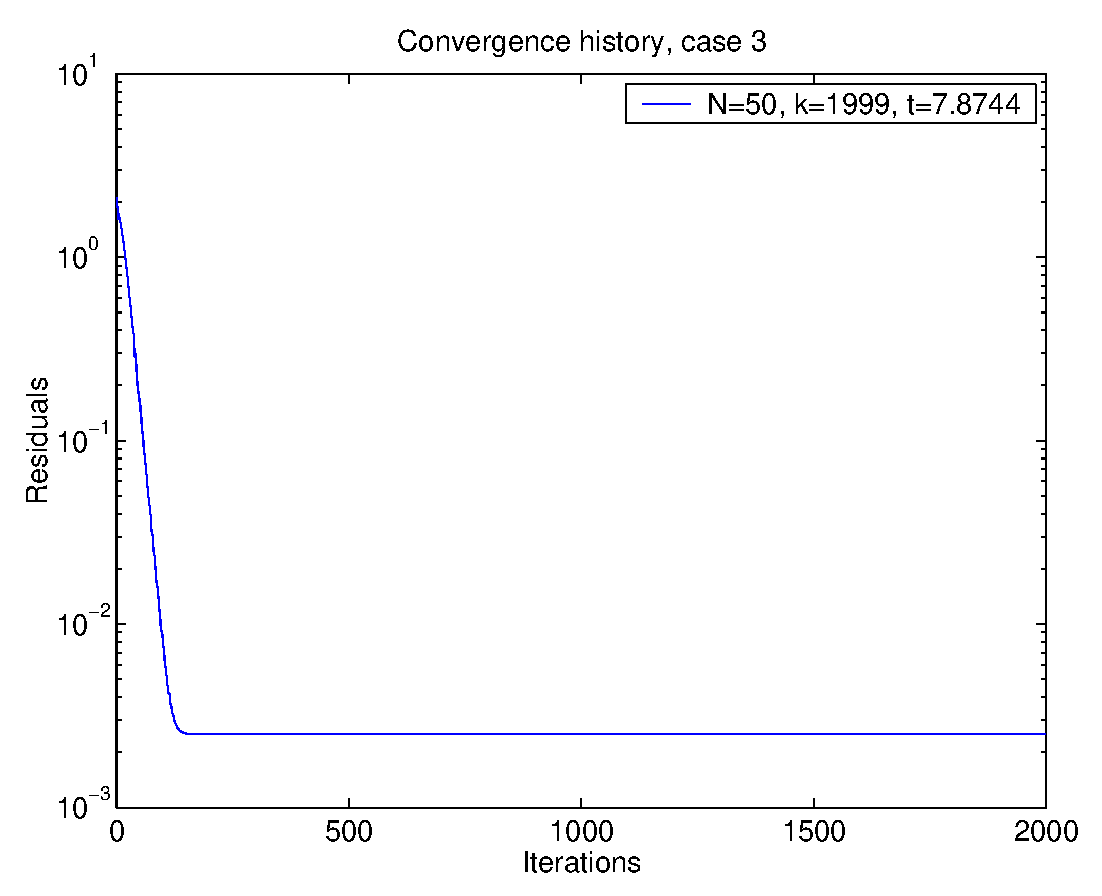
\includegraphics[scale=0.35]{eps/tscheb3.eps}\hfill\includegraphics[scale=0.35]{eps/tscheb4.eps} \\
\includegraphics[scale=0.35]{eps/tscheb5.eps}\hfill {}
\caption{Numerische Resultate f"ur das Modellproblem auf einem $50 \times 50$-Gitter}
\end{figure}
